\chapter{LITERATURE REVIEW}
\section{Introduction}This chapter looks at the existing research and tech behind building the LexiFlow system. It kicks off with a quick tour of second language acquisition theories, the kind that shape pretty much any language learning tool. Then it digs into what makes Mandarin tricky as a symbolic language, and checks out the current methods and systems already out there. Basically, this review sets the theoretical groundwork and points to the gaps LexiFlow wants to fill.
\section{Theories of Second Language Acquisition}
\subsection{Krashen's Input Hypothesis}Krashen's Input Hypothesis~\citep{krashen1985} is one of the main theoretical pillars holding up LexiFlow. The claim? Language acquisition kicks in when learners run into comprehensible input. By comprehensible input, we mean material sitting just a notch above where the learner currently is (i+1). Grammar, in this view, gets picked up naturally through exposure rather than someone drilling rules into you. It's basically how kids learn their first language, soaking it up by listening and interacting with words in real context. Picture a student at HSK 2 who can manage simple chats about everyday stuff. Krashen's "i+1" idea says this person learns best when they bump into content around HSK 3 level material that brings in fresh vocabulary and grammar while still keeping enough familiar bits around to stay understandable. {Table~{\ref{tab:hsk2}}} lays out the vocabulary requirements for each HSK (Hanyu Shuiping Kaoshi) level, the standardized Chinese proficiency exam. Each level stacks on top of the last one. Take a student at HSK 2, who's got 300 words under their belt; HSK 3 bumps that up to 600. \begin{table}[h]
    \centering
    \caption{HSK 2.0 Vocabulary Requirements \citep{hsk2}}\label{tab:hsk2}
    \begin{tabular}{@{}lll@{}}
        \toprule
        \textbf{Current Level (i)} & \textbf{Vocabulary Size} & \textbf{Cumulative Words} \\
        \midrule
        HSK 1                      & 150 words                & 150 words                 \\
        HSK 2                      & 150 words                & 300 words                 \\
        HSK 3                      & 300 words                & 600 words                 \\
        HSK 4                      & 600 words                & 1,200 words               \\
        HSK 5                      & 1,300 words              & 2,500 words               \\
        HSK 6                      & 2,500 words              & 5,000 words               \\
        \bottomrule
    \end{tabular}
    \smallskip

\end{table} Plenty of studies back this up. ~\citet{RODRIGO2004} showed that heavy exposure to comprehensible input through reading led to way bigger vocabulary gains than the old-school instruction approach. And~\citep{krashen2017} found students fed lots of comprehensible input beat the grammar-translation crowd, even on tests of grammar itself.
With Mandarin though, the real problem is finding content that's actually engaging and that you can understand. Figure~\ref{fig:mandarin_dilemma} sums up the whole Mandarin learning dilemma LexiFlow is trying to fix. It's a YouTube video that counts as comprehensible input, Chinese characters running along the bottom as subtitles. But here's the catch, those subtitles come with no Pinyin guide whatsoever, so they're basically useless to beginner and intermediate learners who haven't memorized thousands of characters yet. The video also isn't pitched at any particular skill level, and since the subtitle option is turned off, none of the existing translation tools work on it. Figure~\ref{fig:mandarin_pinyin} shows what good subtitles look like, hand-made by a YouTube channel. Trouble is, doing that takes forever and a ton of effort, which makes it pretty rare and leaves you with a tiny library to work from. \begin{figure}[ht]
    \centering
    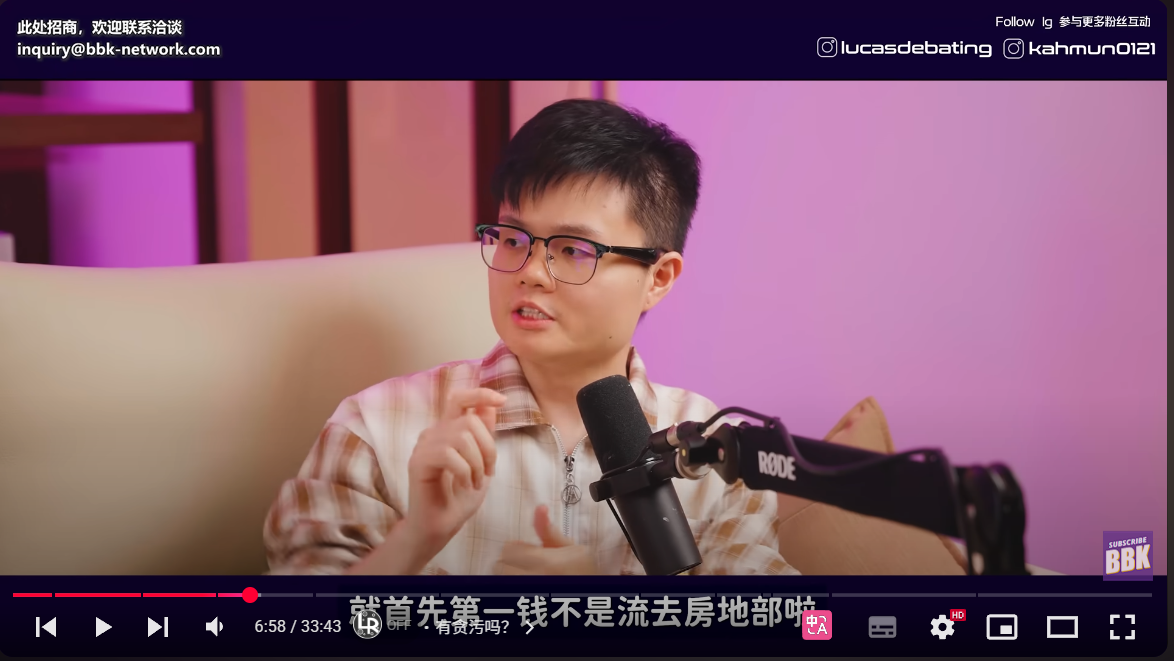
\includegraphics[width=0.8\textwidth]{./figs/yt.png}
    \caption{Example of Mandarin Learning Dilemma}
    \label{fig:mandarin_dilemma}
\end{figure} \begin{figure}[ht]
    \centering
    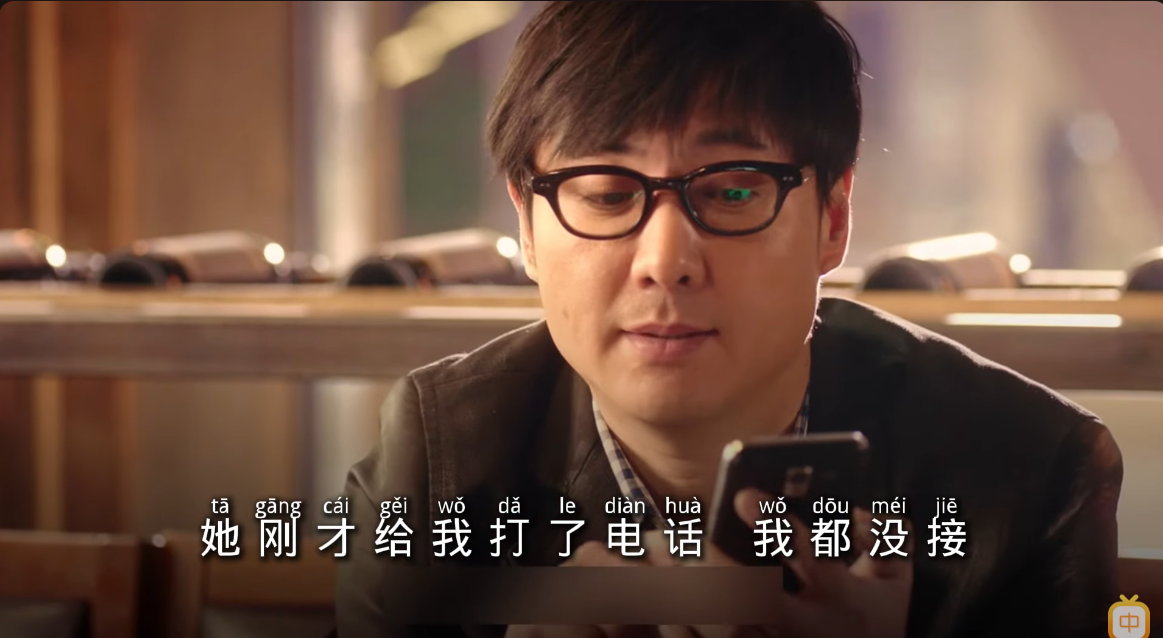
\includegraphics[width=0.8\textwidth]{./figs/yt2.png}
    \caption{Example of Proper Subtitles with Pinyin}
    \label{fig:mandarin_pinyin}
\end{figure}
\subsection{Multimedia Learning Theory}Mayer's Multimedia Learning Theory~\citep{Mayer_2009} is another key pillar holding up LexiFlow's approach. The idea is simple. People learn more deeply from words paired with pictures than from words on their own, notably when the verbal and visual pieces show up but also rather than one after the other. Work by~\citet{jones2002} found vocabulary retention jumped 42\% when learners could see written text alongside visual annotations, versus text alone. For character-based languages,~\citet{shen2010} noticed that multimedia presentations linking spoken words, written characters, and visual cues bumped character recognition up 35\% over the usual methods. And~\citet{li2022} showed Mandarin learners did better on listening comprehension when subtitles were available during practice. That backs up what LexiFlow does, offering multimodal input through its synced transcription and translation interface.
\section{Challenges of Mandarin as a Symbolic Language}
\subsection{Character Recognition and Sound Awareness}Mandarin works differently from alphabetic languages, where the written symbols map straight onto sounds. Its logographic system throws new problems at learners. Work by~\citet{everson2011} found that Western learners need to see a Chinese character roughly 17 times before they reliably recognize it, against just 8 exposures for words in alphabetic languages. The characters are visually dense, and that's where the extra mental load comes from. This gap between Mandarin's written and spoken forms is what linguists call the `orthographic barrier'~\citep{shen2007}. It really slows learning down. Students know spoken words but can't link them to the written shapes they keep running into. Pinyin acts as a bridge here, though~\citet{ye2013} found 76\% of intermediate learners still struggled moving from pinyin-supported texts to character-only ones. LexiFlow tackles this by keeping audio, pinyin, and characters tied together across real content, so learners slowly build character recognition while still getting meaning through the sounds.
\subsection{Tonal Perception and Production}Another big hurdle the literature points to? Mandarin being tonal. Work by~\citet{wang1999} found that adult learners coming from non-tonal languages need targeted practice before they can hear and say the four tones correctly. Without that explicit tonal training, beginners in their study still scored under 40\% on comprehension, even after 200 hours sitting in class. Textbooks usually do tones in isolation, or inside these neat, pre-built dialogues. That's just not how people actually talk. LexiFlow gives students real content with pinyin annotations marked for tone, so they can sharpen their ear naturally.
\section{Current System Analysis}The way students currently study from real content? It's tough on everyone, learners and teachers alike. From what we saw at UTM, plus talking with Mandarin educators, the whole thing takes a ton of manual work. And the content libraries stay pretty limited.
\subsection{Problem with Current System}The way people bring real Mandarin content into their learning right now? It's painfully manual, eats up resources, and that caps both how much material exists and how good it is. Look at the AS-IS swimlane diagram ({Figure {\ref{fig:as_is}}}). The whole item kicks off with an instructor or some motivated student hunting around for authentic content that might task That hunt takes forever, and half the time what you find doesn't even match the right proficiency level. \begin{figure}[ht]
    \centering
    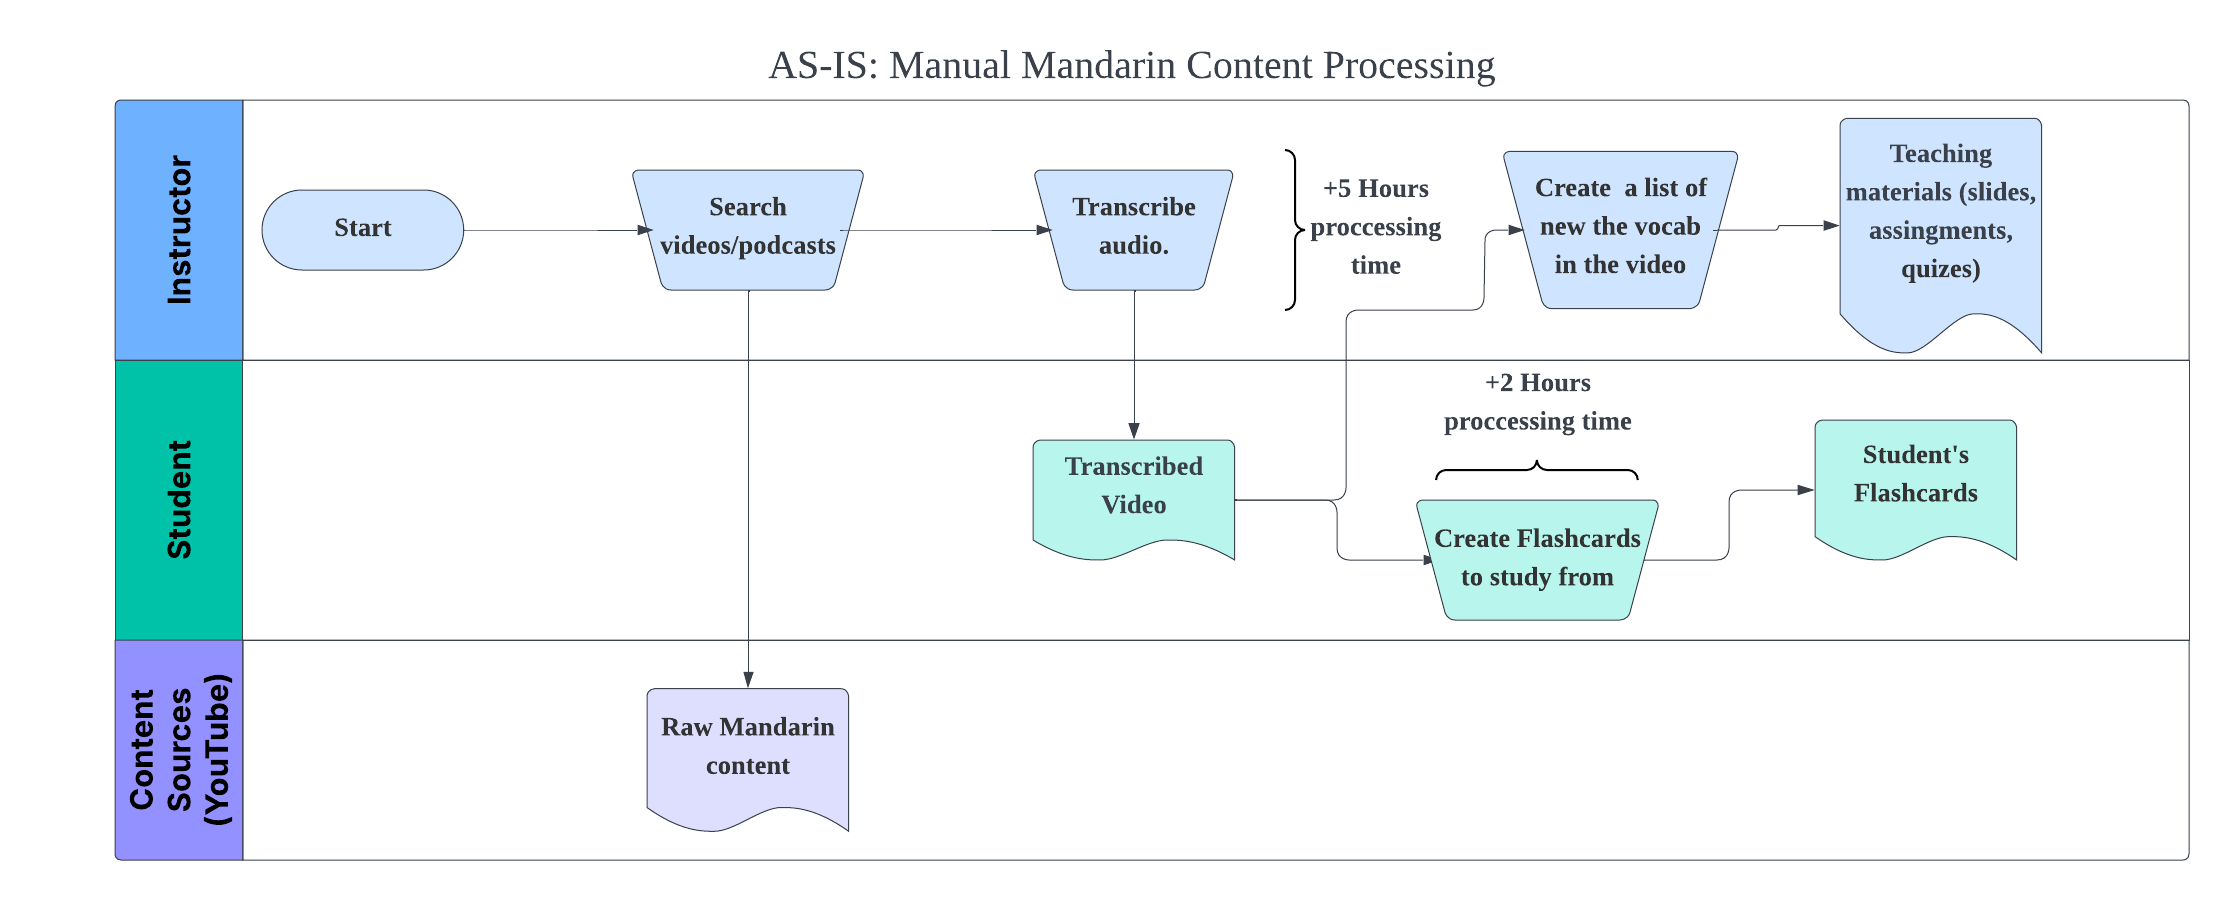
\includegraphics[width=1\textwidth]{./figs/AS-IS.PNG}
    \caption{AS-IS Swimlane Diagram}
    \label{fig:as_is}
\end{figure} So you've found something. Now the real headache starts. Instructors have to transcribe the Mandarin audio by hand, add pinyin annotations, and translate everything, and a measly 5-minute video can swallow 8 to 10 hours. That kind of grind keeps the content pile small. And students who go it alone? Without instant feedback, comprehension gets even harder. Whatever materials come out of all this usually don't have synced timestamps, the thing that'd let learners line up spoken words with what's written. The content also tends to show up stripped of context, so beginners can't really follow it. Which basically makes it useful only for advanced students (in my view).
\subsection{Proposed Solution}LexiFlow tackles these slowdowns by automating the parts of content processing that eat up the most time, all while keeping quality high. The TO-BE swimlane diagram ({Figure {\ref{fig:to_be}}}) lays it out. Basically, the system builds a cleaner workflow that helps instructors and students alike. \begin{figure}[ht]
    \centering
    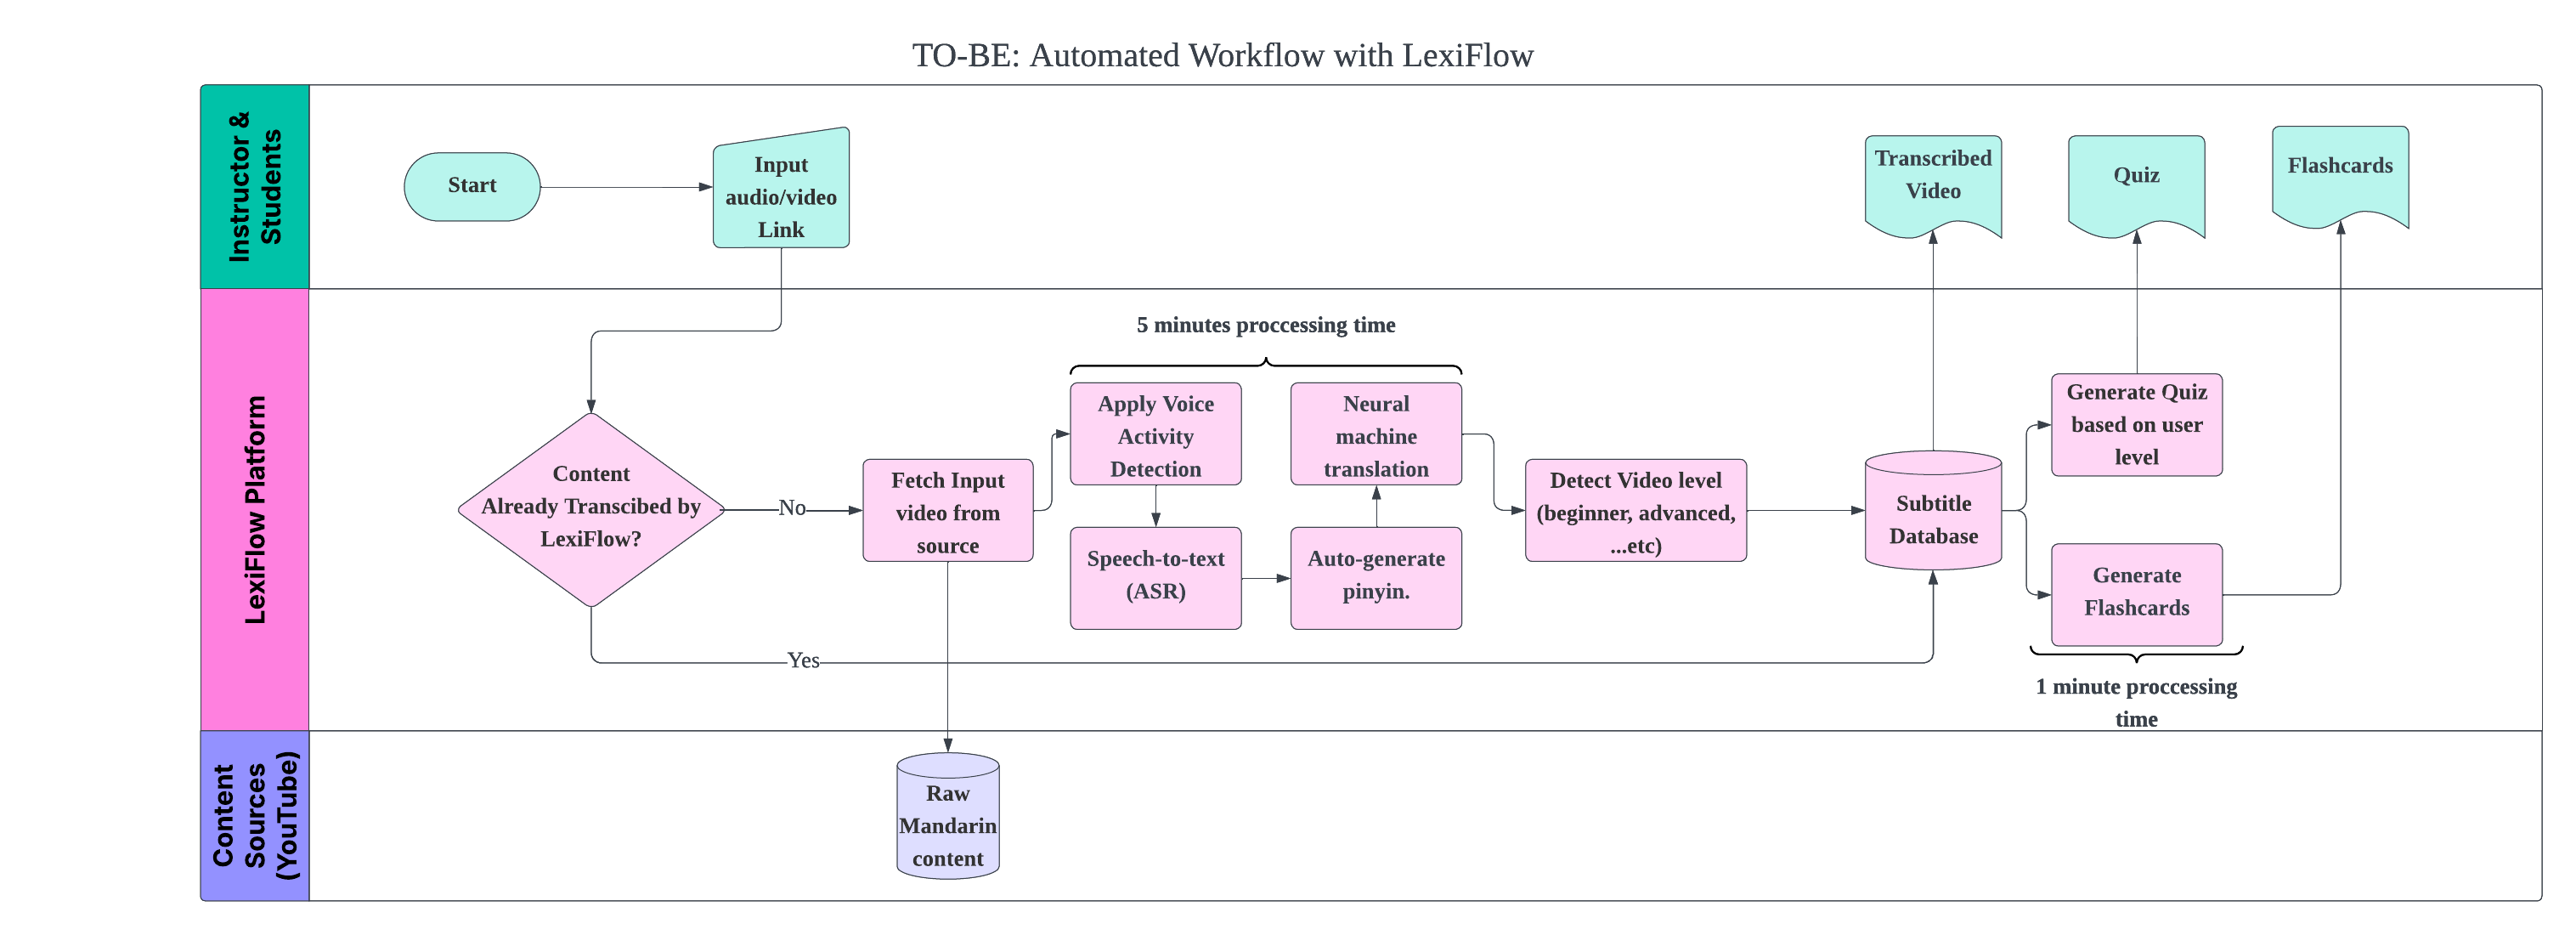
\includegraphics[width=1\textwidth]{./figs/TO-BE.PNG}
    \caption{TO-BE Swimlane Diagram}
    \label{fig:to_be}
\end{figure} It starts when users upload real Mandarin audio or video. From there, LexiFlow chops the content into sentence-sized chunks using voice activation detection. Each chunk then runs through its own pipeline, automatic speech recognition handles the transcription, pinyin gets generated, and neural machine translation takes care of the English. Everything that's been processed lands in an indexed database, so there's no redundant labor when different users pull up the same material. And that's kind of the clever part. The library grows on its own, shaped by what people actually want and want
\subsection{Comparison of Similar Video-Based Learning Platforms}A few platforms have tried building language learning around video, and the results have been mixed. FluentU, looked at by~\citet{xu2020}, shows that hand-picked video libraries paired with interactive transcripts help listening comprehension more than the old-school audio drills. But the same study flagged a headache content limitations. Advanced learners kept griping about there not being enough variety. Figure~\ref{fig:fluentu-browse} shows the FluentU platform's video browse page and its curated library. Figure~\ref{fig:fluentu} gives an example of a single video, complete with interactive transcripts and vocabulary tools. \begin{figure}[H]
    \centering
    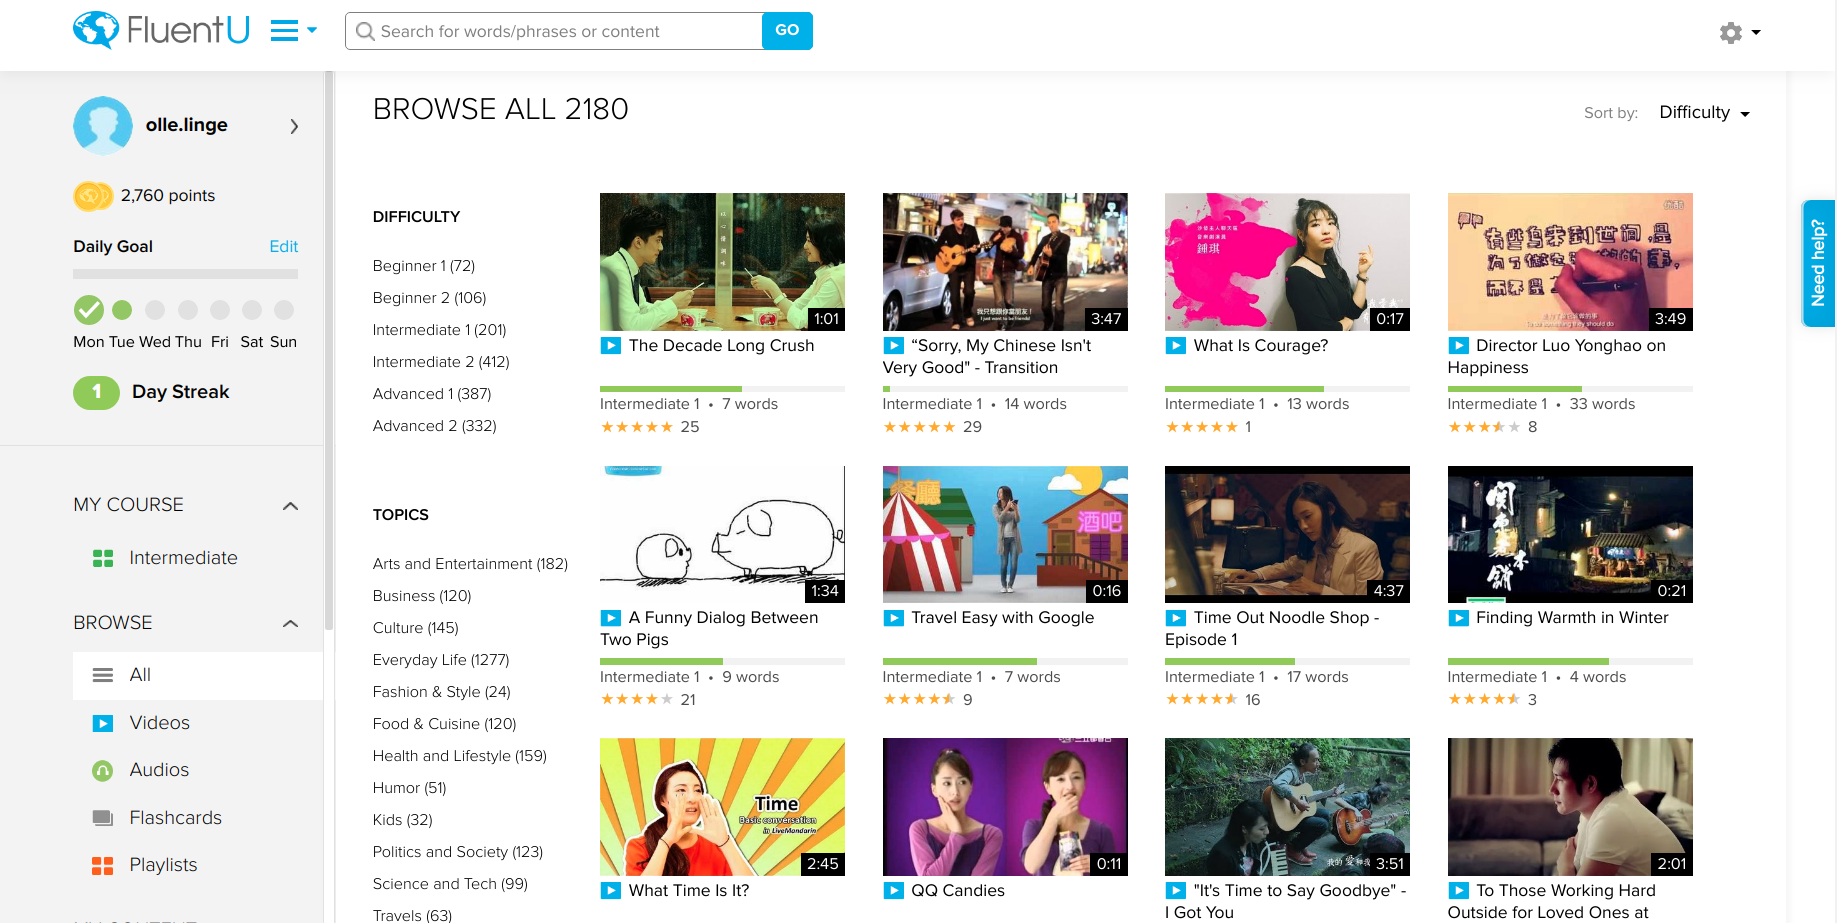
\includegraphics[width=1\textwidth]{./figs/fluentu-video-browse.png}
    \caption{FluentU Platform Video Browse Page}
    \label{fig:fluentu-browse}
\end{figure} \begin{figure}[H]
    \centering
    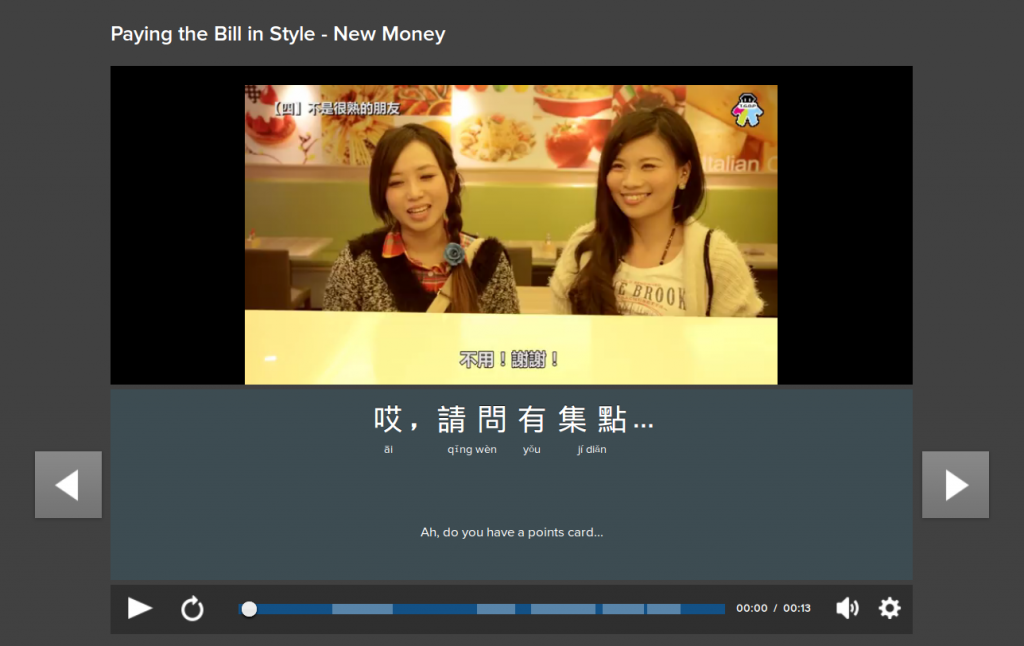
\includegraphics[width=1\textwidth]{./figs/fluentu-video.png}
    \caption{FluentU Platform Video Example}
    \label{fig:fluentu}
\end{figure} LanguageReactor, which used to go by Language Learning with Netflix and was examined by~\citet{dizon2021}, is a free browser extension. It lets you overlay bilingual subtitles on top of Netflix and YouTube videos. You get basic stuff for looking up vocabulary and playing back sentence by sentence. The catch? It leans entirely on subtitles that already exist and doesn't make its own, so quality jumps all over the place. Figure \ref{fig:language-reactor-settings} shows the LanguageReactor settings page where you can tweak subtitle options. Figure~\ref{fig:language-reactor} shows a video on the platform with bilingual subtitles and vocabulary tools. \begin{figure}[H]
    \centering
    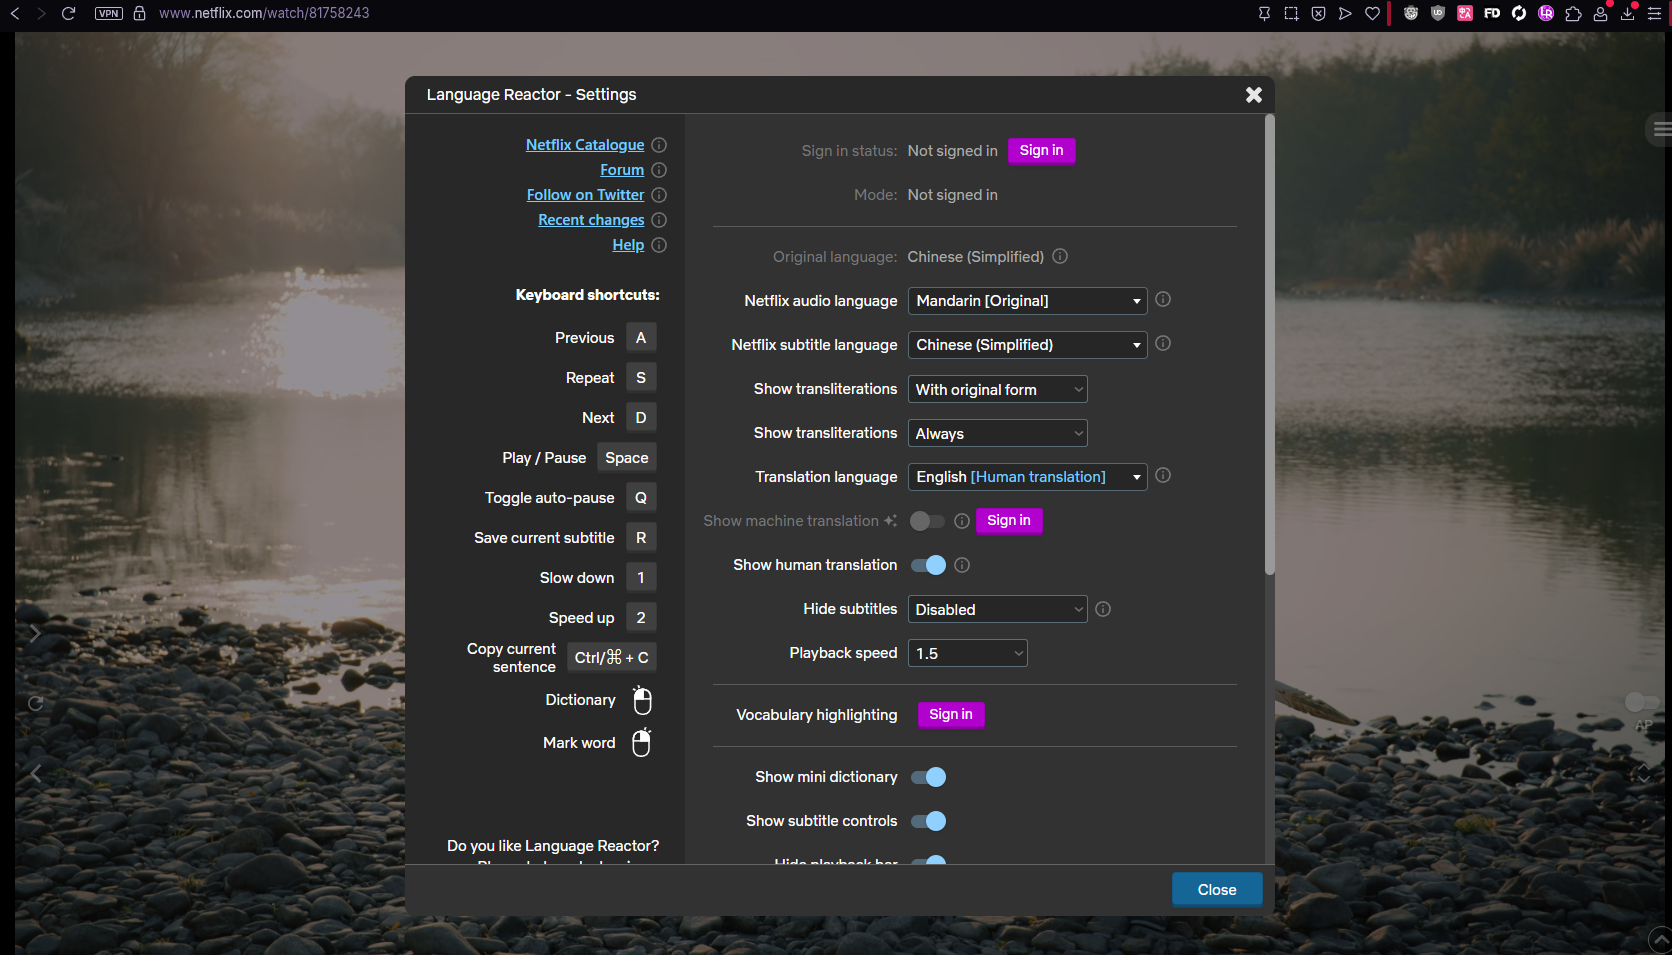
\includegraphics[width=1\textwidth]{./figs/lang_reactor-settings.png}
    \caption{LanguageReactor Settings Page From Netflix}
    \label{fig:language-reactor-settings}
\end{figure} \begin{figure}[H]
    \centering
    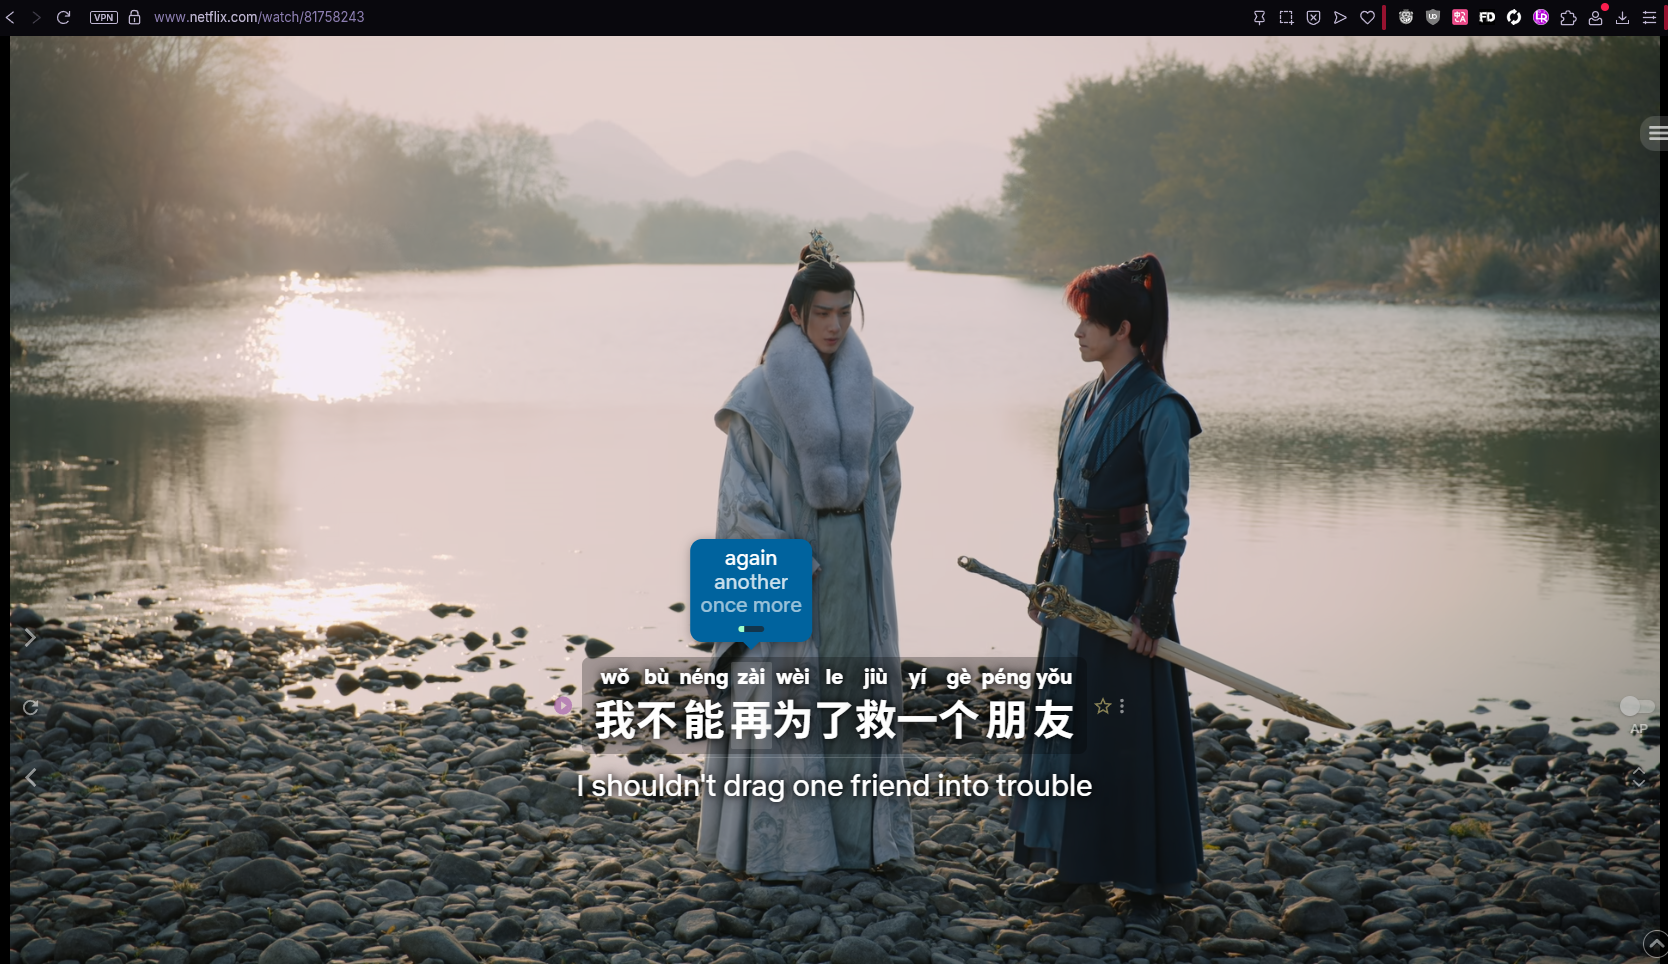
\includegraphics[width=1\textwidth]{./figs/lang_reactor.png}
    \caption{LanguageReactor Example From Netflix}
    \label{fig:language-reactor}
\end{figure} Yabla's a subscription service with a curated video library and interactive features baked in. Work by~\citet{pujadas2024} found that Yabla's setup leads to better vocabulary retention than just watching videos the normal way. The interface is clean and the content's well produced, sure, but the library itself is tiny and short on range. One upside: the platform builds its own custom subtitles instead of pulling everything from third parties, which makes them more accurate than what LanguageReactor offers. Figure \ref{fig:yabla-browse} shows Yabla's video browse page and its curated library. Figure~\ref{fig:yabla} shows a single video with its playback controls and vocabulary tools. Those controls let you slow segments down or replay them, which helps comprehension and retention stick. \begin{figure}[H]
    \centering
    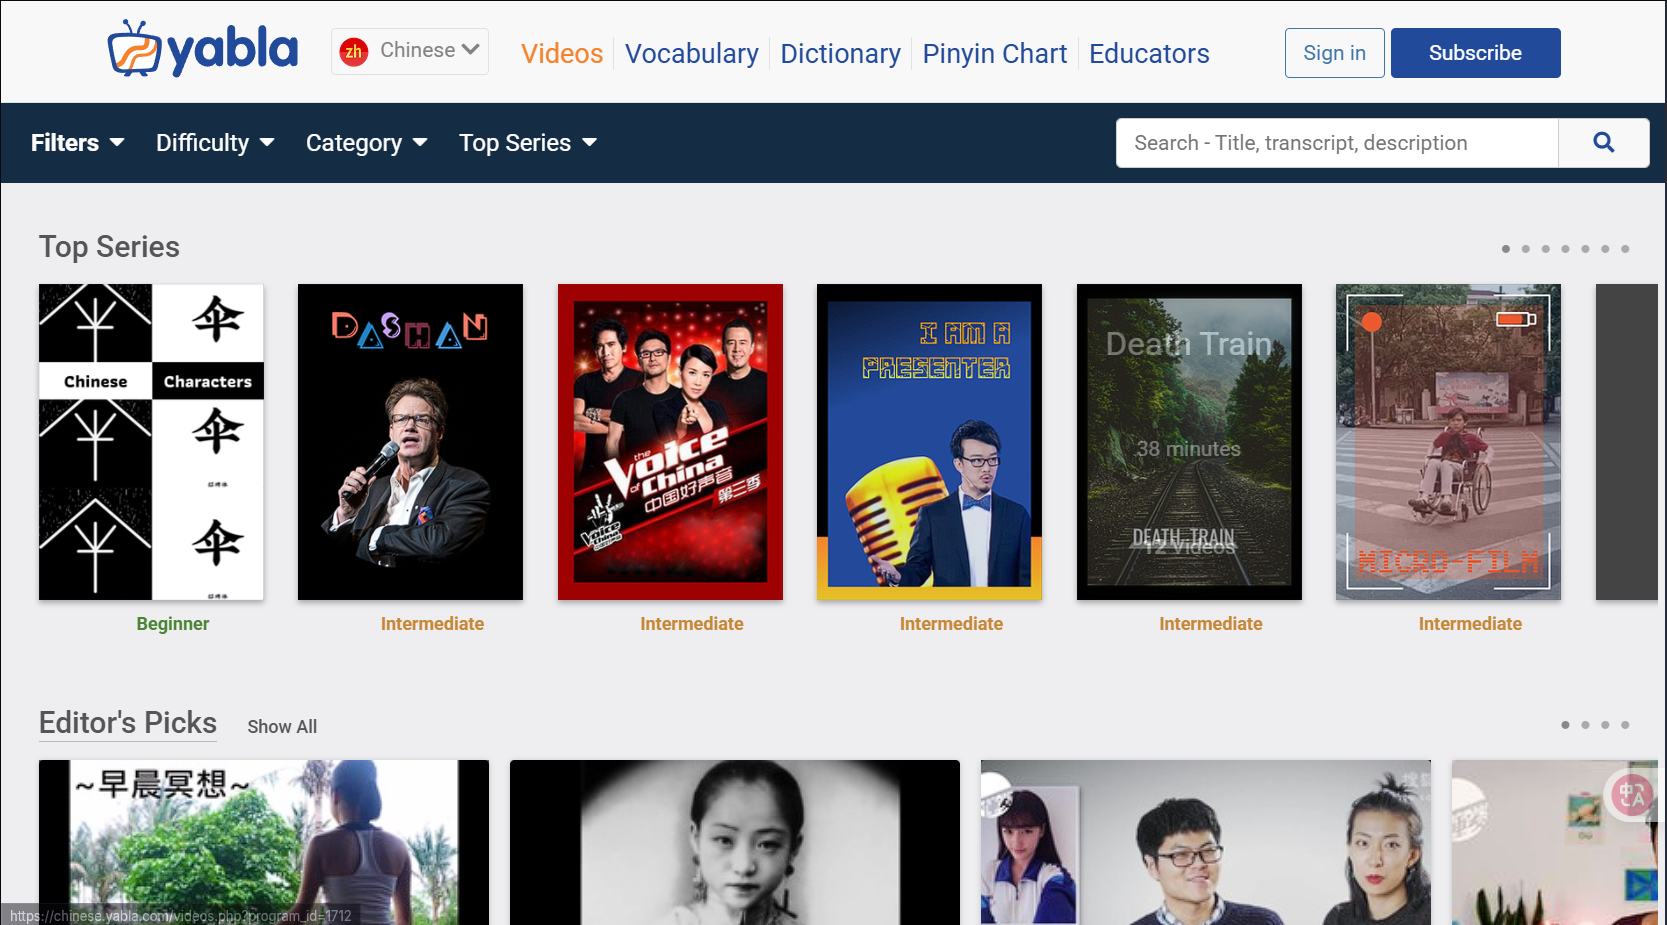
\includegraphics[width=1\textwidth]{./figs/yabla-video_browse.png}
    \caption{Yabla Platform Example}
    \label{fig:yabla-browse}
\end{figure} \begin{figure}[H]
    \centering
    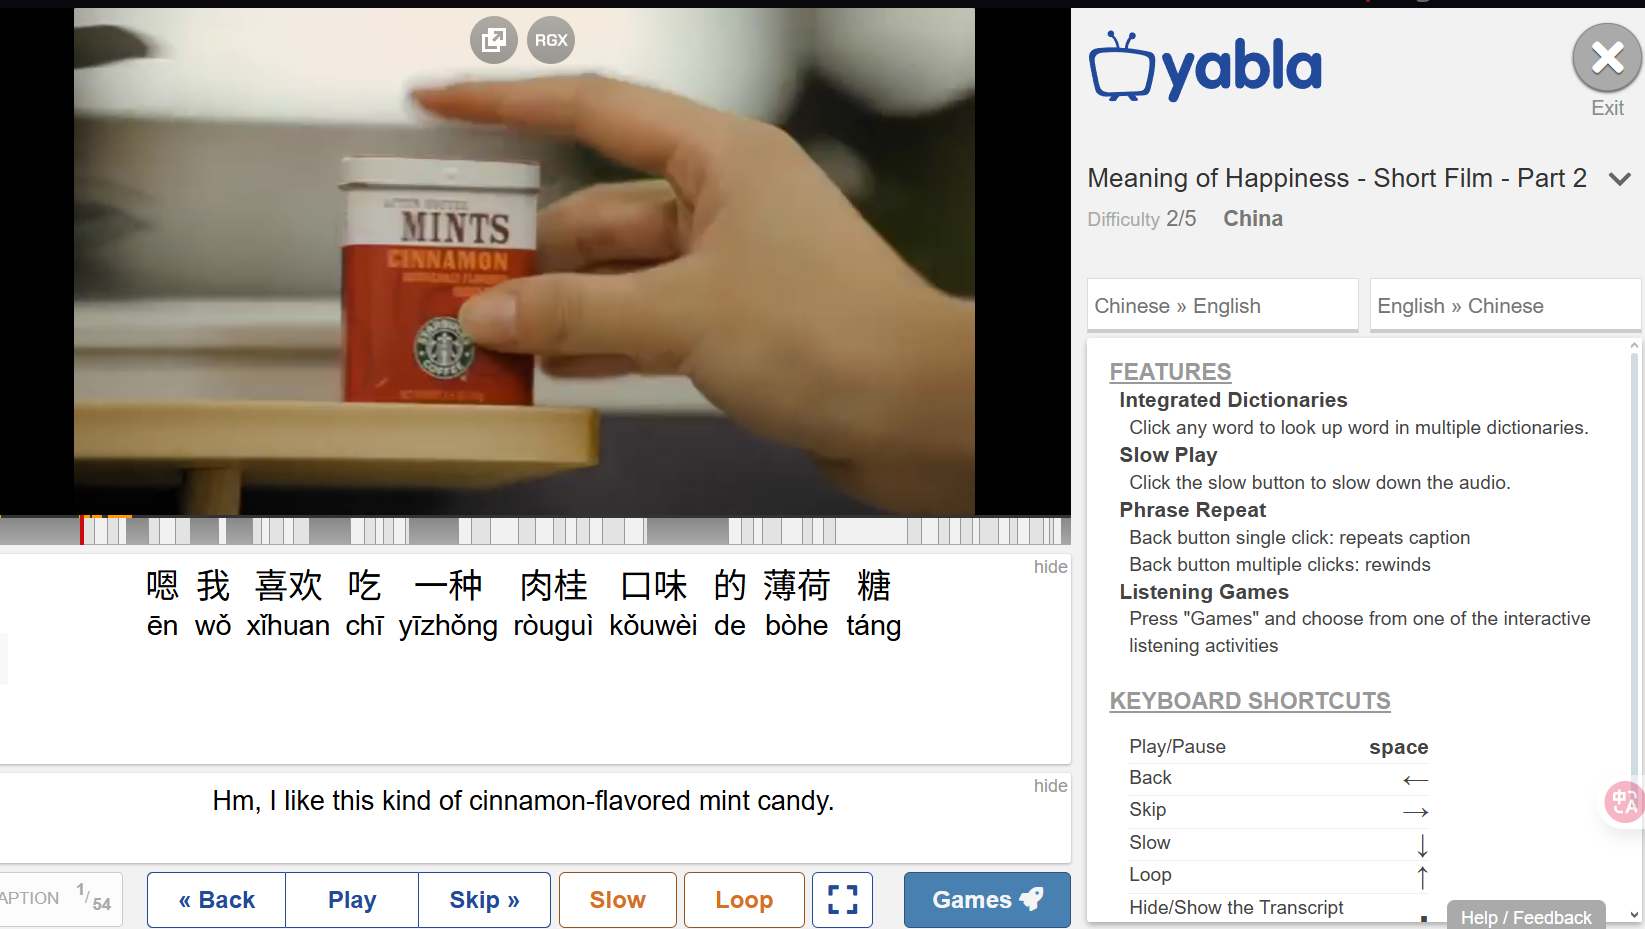
\includegraphics[width=1\textwidth]{./figs/yabla.png}
    \caption{Yabla Platform Video Example}
    \label{fig:yabla}
\end{figure}
All three existing systems use video for language learning, but they tackle the same basic difficulty in different ways, giving learners engaging, authentic content with solid language support. Every one of them leans on subtitles that already exist or got made by hand {as shown in table~{\ref{tab:feature_comparison}}}. That's a real bottleneck. And it hits Mandarin learners hardest, since there's just way less subtitled content out there compared to French or German. \begin{table}[h]
    \centering
    \caption{Language Learning Platform Feature Comparison}
    \scalebox{0.85}{
        \begin{tabular}{lllll}
            \toprule
            \textbf{Feature} & \textbf{Lang.Reactor} & \textbf{FluentU} & \textbf{Yabla}    & \textbf{{LexiFlow*}}          \\
            \midrule
            Content Source   & YT/Netflix subs       & Closed library   & Curated videos    & {Any Mandarin audio}          \\
            Pinyin Support   & Word-level            & Full             & Full              & {Full}                        \\
            Processing       & Existing subs         & Manual           & Manual            & {Auto segmentation}           \\
            Growth           & Subtitle-limited      & Slow manual      & Slow manual       & {Exponential User-driven}     \\
            Efficiency       & High                  & Low              & Low               & {Medium}                      \\
            Cost             & Freemium              & Sub only         & Sub only          & {Freemium}                    \\
            Personalization  & Basic vocab           & Adaptive quiz    & Playback controls & {Interest-based} \\
            \bottomrule
        \end{tabular}
    }
    \label{tab:feature_comparison}

    \begin{flushleft}
        \small * Proposed solution
    \end{flushleft}
\end{table} LexiFlow does something different. It generates subtitles automatically for any Mandarin audio or video, so you don't need them sitting around beforehand. The content library can balloon fast as more people upload and process their own stuff, which beats the slow, manual updates other platforms depend on. There's a freemium setup too, core features are free, while premium folks get extras like flashcards and quizzes built just for them. It also pays attention to what you're into and the words you've saved, then uses that to suggest content you'll truthfully care about and put together study materials made for you. Honestly, that's what makes the whole thing click.
\section{Technologies for Video-Based Learning Platform}
\subsection{Voice Activity Detection and Sentence Segmentation}VAD systems sit at the heart of modern voice recognition. They spot speech and non-speech segments frame by frame, then kick off whatever comes next, speech recognition, augmentation, endpointing. For Mandarin in particular,~\citet{pan2025} found something compelling splitting speech into smaller chunks with the Silero-VAD~\citep{sileroVAD} model beat general-purpose systems at catching boundaries. Sentence-level segmentation worked better than chewing through longer stretches all at once. That backs up LexiFlow's segment-by-segment approach.
\subsection{Automatic Speech Recognition for Mandarin}Automatic Speech Recognition (ASR) began with crude systems that responded to a handful of sounds, and over time it's grown into something that handles spoken language fluently. The push to automate easy tasks built around human-machine interaction is what's driven so much interest in ASR. OpenAI's Whisper~\citep{radford2023robust} is an ASR system trained on 680,000 hours of multilingual, multitask supervised data pulled from the web. The architecture itself is a straightforward end-to-end design, built as an encoder-decoder Transformer. It transcribes speech and identifies languages with high accuracy, even when the audio is noisy or otherwise tricky. Now, for educational uses. ~\citet{sutomo2024} found that even at character error rates of 6--10\%, learners said ASR-generated transcripts were quality enough to follow along. That tells us current ASR has hit a point where it's genuinely usable in language learning tools like LexiFlow.
\subsection{Neural Machine Translation}Neural Machine Translation (NMT) has done a lot to boost the quality and reliability of automated translation. Per~\citet{hassan2018}, today's NMT systems have hit human parity for Chinese-English news content, which is kind of a big deal for cross-lingual work. ~\citet{barrault2023seamless} smoothM4T v2 is Meta's massively multilingual, multimodal translation model. It's built to deliver high-quality, real-time translation across speech and text in nearly 100 languages. The v2 release runs on the UnitY2 architecture, with hierarchical character-to-unit upsampling and non-autoregressive decoding. Here's what matters for LexiFlow. ~\citet{gary2024} found that even when translations had small slips, showing learners both the source and the machine version improved comprehension over source-only. So LexiFlow's whole approach, pairing translations with the original Mandarin, holds up.
\subsection{NoSQL Database Implementation}Modern video-learning platforms get a lot out of NoSQL databases. They're flexible, they scale, and honestly they just perform better than the old relational setups for this kind of thing. SQL databases want everything structured. NoSQL doesn't care about schemas, which makes it a solid fit for messy, ever-changing stuff like video metadata, user interactions, and learning analytics that maintain shifting around. Document stores like MongoDB are great at wrangling unstructured and semi-structured data, so storing and pulling back multimedia content, user profiles, and session logs stays painless. The distributed setup keeps things available and lets you scale sideways as your users and content pile up. Key-value and wide-column databases speed up reads and writes for real-time analytics. And graph databases? They're solid for mapping out how concepts, users, and learning materials all connect.
\section{Summary}So this literature review pulled together a handful of findings that shape how LexiFlow gets built. To start, Krashen's Input Hypothesis and Multimedia Learning Theory turned out to be solid theoretical ground for LexiFlow's whole approach. From there I looked at Mandarin's symbolic writing system and the odd challenges it throws up. The current crop of language learning apps and where they fall short got a close look too. And the review wrapped with the recent jumps in Voice Activity Detection, Automatic Speech Recognition, and Neural Machine Translation, plus a discussion of which models the system's truthfully planning to put to work % \begin{enumerate}[label= (\alph*)]
% \item Krashen's Input Hypothesis and Multimedia Learning Theory provide strong theoretical foundations for LexiFlow's approach of making authentic content comprehensible through technological scaffolding. % \item Mandarin's logographic writing system creates unique challenges that require specialized technological solutions connecting spoken and written forms. % \item Current language learning applications tells us the value of authentic video content but suffer from critical limitations in content availability and flexibility. % \item Recent advances in Voice Activity Detection, Automatic Speech Recognition, and Neural Machine Translation have reached sufficient maturity to support educational applications with high accuracy. % \item Sentence-level processing approaches offer significant advantages in both computational efficiency and accuracy compared to whole-file processing. % \item Interest-driven learning consistently shows superior engagement and outcomes compared to prescribed content approaches. What this review honestly does is show two things at once: that LexiFlow's approach to Mandarin learning through efficient processing of authentic content is genuinely needed, and that it's actually doable. The next chapter digs into how all of this gets put into practice inside the LexiFlow system (if you think about it).
